\documentclass{article}

% Language setting
\usepackage[polish]{babel}

% Set page size and margins
\usepackage[a4paper,top=2cm,bottom=2cm,left=3cm,right=3cm,marginparwidth=1.75cm]{geometry}
\usepackage[T1]{fontenc}

% Useful packages
\usepackage{amsmath}
\usepackage{graphicx}
\usepackage{subcaption}
\usepackage[colorlinks=true, allcolors=blue]{hyperref}
\usepackage{float}
\usepackage{listings}

\title{CAD/CAE - zadanie 6}
\author{Iwo Szczepaniak}

\begin{document}
\maketitle

\section{Sposób znaleznienia punktów startowych}
Do przygotowania punktów startowych posłużyłem się pętlą, wewnątrz której końcowe parametry danej iteracji stają się parametrami startowymi kolejnej. Dzięki temu udało się osiągnąć znaczną poprawę w aproksymacji funkcji.

\section{Zmiany w kodzie}
W ramach zadania zmodyfikowano kod źródłowy w celu trenowania sieci neuronowej do aproksymacji funkcji B-spline. Poniżej przedstawiono kluczowe fragmenty implementacji:
\begin{verbatim}
function NNtrain()
    ...
    % Training
    a1=1.0; b1=1.0; c1=1.0; d1=1.0;
    a2=1.0; b2=1.0; c2=1.0; d2=1.0;
    a3=1.0; b3=1.0; c3=1.0; d3=1.0;
    eta1=0.1; eta2=0.1; eta3=0.1;
    
    num_epochs = 500;
    for epoch = 1:num_epochs
        for j=1:ndataset
            i=floor(r(j));
            if(i==0)
                i=1;
            end
            % Old training steps, but for each epoch
            % ...
        end
    end
    
    % Display learned parameters
    disp(['a1 = ', num2str(a1), ', b1 = ', num2str(b1), ', c1 = ', num2str(c1), ', d1 = ', num2str(d1)]);
    disp(['a2 = ', num2str(a2), ', b2 = ', num2str(b2), ', c2 = ', num2str(c2), ', d2 = ', num2str(d2)]);
    disp(['a3 = ', num2str(a3), ', b3 = ', num2str(b3), ', c3 = ', num2str(c3), ', d3 = ', num2str(d3)]);
end
\end{verbatim}

\section{Wyliczone parametry}
Po przeprowadzeniu treningu sieci neuronowej, uzyskano następujące parametry:
\begin{itemize}
    \item $a1 = 0.95251$, $b1 = 0.89256$, $c1 = 0.0559$, $d1 = -0.049677$
    \item $a2 = 2.851$, $b2 = -0.26152$, $c2 = 2.6766$, $d2 = -1.2066$
    \item $a3 = 3.2571$, $b3 = -0.28923$, $c3 = 2.9184$, $d3 = -1.1524$
\end{itemize}

\newpage
\section{Wyniki symulacji}
Przeprowadzona symulacja pokazuje aproksymację funkcji B-spline za pomocą wytrenowanej sieci neuronowej. Poniżej przedstawiono wyniki w postaci wykresów:

\begin{figure}[H]
    \centering
    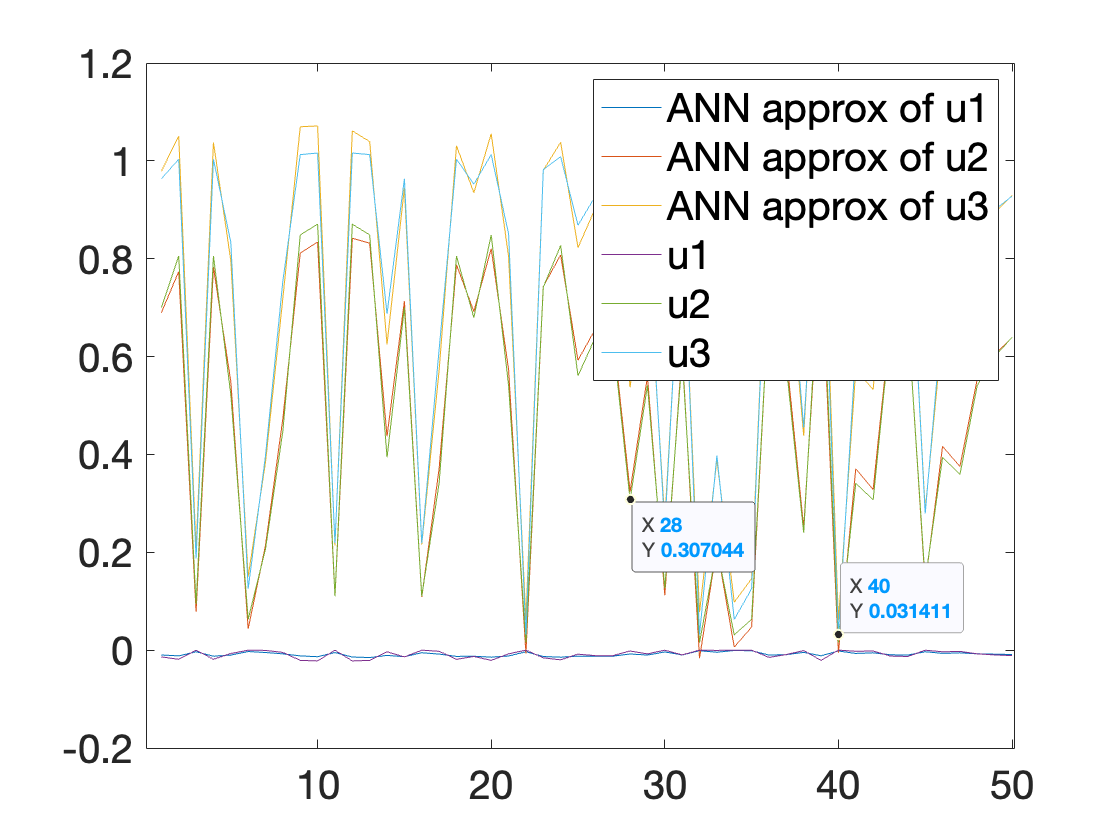
\includegraphics[width=0.8\linewidth]{params_plot.png}
    \label{fig:params-plot}
\end{figure}

\begin{figure}[H]
    \centering
    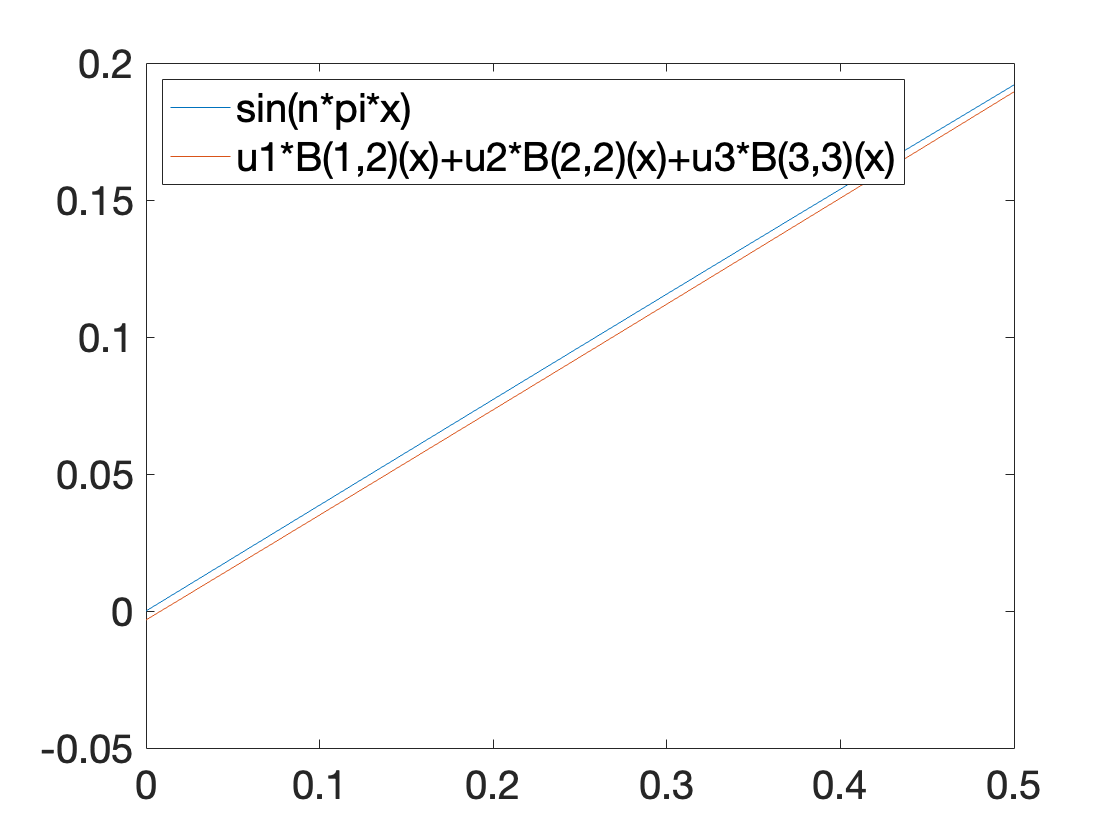
\includegraphics[width=0.8\linewidth]{approx_plot.png}
    \label{fig:approx-plot}
\end{figure}

\begin{figure}[H]
    \centering
    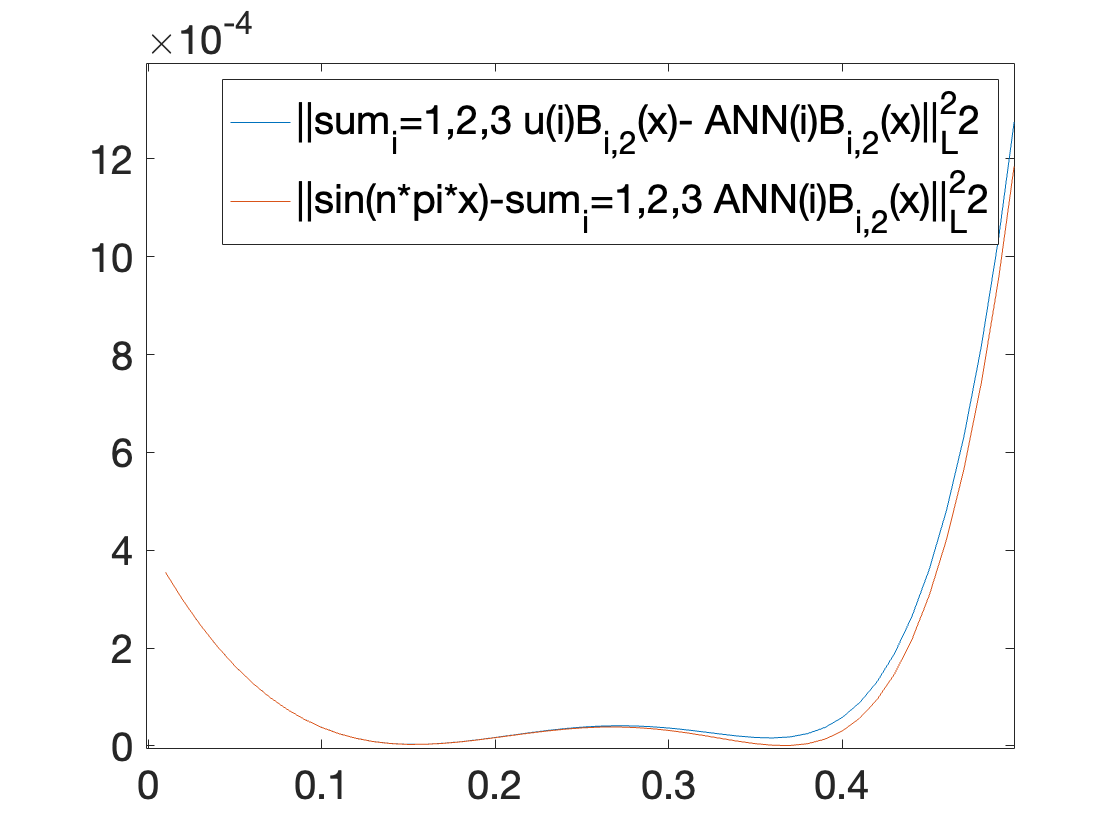
\includegraphics[width=0.8\linewidth]{approx_plot_2.png}
    \label{fig:approx-plot}
\end{figure}

\end{document}

